\section{Lecture 2}
Supervised learning of behaviors and imitation learning
\subsection{Part 1}
\subsubsection{Notation and Context}
Given an observation $o$, our goal is to find a policy $\pi_\theta(a_t|o_t)$ that maps an observation to an action at a time $t$.
\begin{itemize}
    \item $\textbf{o}_t$ - observation
    \item $\textbf{s}_t$ - state (note that this and observation tend to get confounded)
    \item $\textbf{a}_t$ - action
    \item $\pi_\theta(\textbf{a}_t|\textbf{o}_t)$ - policy which can be deterministic or stochastic. We can generalize policies to be stochastic and then if we want a deterministic decision we can pick the most probable outcome.
    \item $\pi_\theta(\textbf{a}_t|\textbf{s}_t)$ - policy (fully observed)    
\end{itemize}

\begin{figure}[htbp]
  \centerline{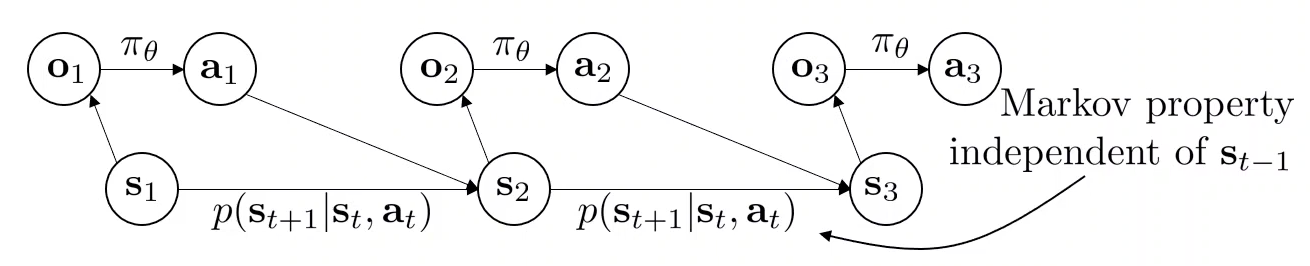
\includegraphics[width=0.75\textwidth]{images/lecture2_grapical_depiction}}
  \caption{Graphical model showing the transition of observations, actions, and states}
  \label{fig:lecture2_grapical_depiction}
\end{figure}

\subsubsection{Imitation Learning}
Imitation learning's goal is to get a policy from looking at observations and actions. Observation and action pairs $(\textbf{o}_t,\textbf{a}_t)$ are taken in as training data and fed into some supervised learning algorithm with the goal of outputting a policy $\pi_\theta(\textbf{a}_t | \textbf{o}_t )$. Imitation learning, or behavior cloning, can be very flawed since it is difficult for it to adapt its knowledge to new situations. The supervised learning model will make a mistake that gets compounded as mistakes will cause it to deviate from the original trajectory. Being in a new trajectory increases the likelihood that the model will make more mistakes.
\\ 
The issue of compounded mistakes is not present in traditional supervised learning since each observation in the data is IID. In a temporal sequence, like a control/reinforcement learning problem, the IID assumption does not hold. This issue can be avoided or mitigated by being smart about the way data is collected and augmented.

\subsection{Part 2}
\subsubsection{Why does behavioral cloning fail?}
If we have a policy $\pi_\theta( \textbf{a}_t | \textbf{o}_t)$ and a data set $(\textbf{o}_t, \textbf{a}_t)$. We can define the probabilities that we pick an action based off of an observation as $p_{data}(\textbf{o}_t)$ and $p_{\pi_\theta} (\textbf{o}_t)$. In this case, as we train using supervised learning, we have the objective function 
\begin{equation}
     \max_\theta \mathbb{E}_{\textbf{o}_t ~ p_{data}(\textbf{o}_t)} [\log \pi_\theta(\textbf{a}_t | \textbf{o}_t)]
\end{equation}
Since there is a difference in the distribution that the model was trained on and the one that it will experience $p_{data}(\textbf{o}_t)$ and $p_{\pi_\theta} (\textbf{o}_t)$, this skews the output. A different objective function can be created using a cost function
\begin{equation}
    c(\textbf{s}_t, \textbf{a}_t) = 
    \begin{cases}
        0 \quad if \textbf{a}_t = \pi^*(\textbf{s}_t)\\ 
        1 \quad otherwise
    \end{cases}
\end{equation}
and we restructure our objective function to be
\begin{align}
  \text{minimize} & \quad \mathbb{E}_{\textbf{s}_t ~ p_{\pi_\theta}(\textbf{s}_t)} [c(\textbf{s}_t, \textbf{a}_t)]
\end{align}
We can analyze how effective behavioral cloning by identifying how likely you are at each time step $t$ in a horizon $T$ to make a mistake. If we assume that for any $\textbf{s} \in D_{train}$, there is a probability $\textbf{prob} [\pi_\theta(\textbf{a} \neq \pi^* (\textbf{s}) | \textbf{s})] \leq \epsilon$. Then if we want to find the expected value of our cost function across all time periods, we can find the below equation. Intuitively, the below equation works by first adding the probability we make a mistake each period to the probability we don't make a mistake on the first step and then every mistake every step after, etc.

\begin{equation}
    \mathbb{E}[\sum_{t} c(\textbf{s}_t, \textbf{a}_t)] \leq \epsilon T + (1-\epsilon)(\epsilon(T-1)) \dots 
\end{equation}

This series increases at a rate $O(\epsilon T^2)$ in the worst case. This is a pessimistic worst case, so in order for behavioral cloning to work in practice, the cost functions and problem structure is usually built in a way to make the state easy to recover from.

\subsection{Part 3}
\subsubsection{Data Collection and Augmentation}
In order to teach the policy to make corrections well, it is important to collect and augment data in way that shows how to do so.
\begin{itemize}
  \item Intentionally add mistakes and corrections to collected data
  \item Augment data to include mistake information.
\end{itemize}

\subsubsection{Model failure types}
Some reasons that a model may fail to fit an expert despite good data collection and augmentation processes could be
\begin{itemize}
  \item Non-Markovian behavior
  \item Multimodal behavior
\end{itemize}
In order to model non-markovian behavior, it is possible to use sequence modelling techniques such as LSTMs and transformers to encode history into a current state. In order to model multimodal behavior, it is important to not add merge distributions together because that could cause an incorrect action. Therefore, a mixture of gaussians can be used.
\\ 
Causal confusion is when a model has too much information and doesn't know exactly what action came from what piece of information.

\subsubsection{Model Methods for Improving Failure}
Mixture of gaussians:
\begin{equation}
  \pi(\textbf{a} | \textbf{o}) = \sum_i w_i N(\mu_i, \Sigma_i)
\end{equation}

\begin{figure}[htbp]
  \centerline{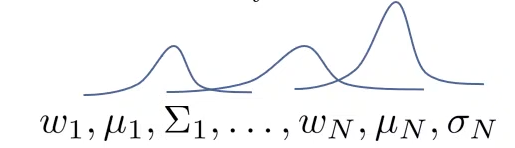
\includegraphics[width=0.75\textwidth]{images/lecture2_gaussian_mixture.png}}
  \caption{Image of an example gaussian mixture and the corresponding distribution}
  \label{fig:lecture2_gaussian_mixture}
\end{figure}

Latent variable models: Conditional variable autoencoders are latent variable models. The idea is to put in anm additional random vector that will tell it which distribution to output.
\\ 
Diffusion models: In diffusion models, random noises is added to a noise and then a model is trained to go through the noisy image and predict what the image looked like before the noise was added. This is extended to reinforcement learning by going through each action, adding noise to it and then training a model that attempts to extract what the original action was.
\\
Discretization: Can discretize the actions by binning them into different steps.

\subsection{Part 4}
\subsubsection{Multi-task learning}
Learning multiple tasks at the same time can make imitation learning easier. For example, we could create a policy that has multiple outcomes it is trying to reach. The goal of this is to increase the coverage of the states in the training data. Random goals can be placed and data collected over them.

\subsection{Part 5}
\subsubsection{Data Collection Strategy}
DAgger algorithm: Dataset  Aggregation. The goal with this algorithm is to get $p_{data}(\textbf{O}_t) = p_{\pi_\theta} (\textbf{o}_t)$.
\begin{itemize}
  \item First: train $\pi_\theta (\textbf{a}_t | \textbf{o}_t)$ from human data $D = \{(\textbf{o}_1, \textbf{a}_1), \dots, (\textbf{o}_N, \textbf{a}_N)\}$
  \item run $\pi_\theta (\textbf{a}_t | \textbf{o}_t)$ to get dataset $D_\pi = \{ \textbf{o}_1, \dots, \textbf{o}_M \}$
  \item Ask human to label $D_\pi$ with actions $\textbf{a}_t$
  \item Aggregate: $D \leftarrow D \cup D_\pi $
\end{itemize}

Basically, the DAgger algorithm has humans retroactively label what the agent should have done and then it adds it to the original dataset.

\subsubsection{Cost functions and reward functions}
The issue with imitation learning is that humans need to provide data. There are multiple limitations with this as humans may not be the best at providing the data for some kinds of actions. Naturally, we shift away from imitation learning into reinforcement learning to alleviate this issue and have the model itself collect data.